\documentclass[../doc.tex]{subfiles}

\begin{document}

\section{Gameplay}

Chaque joueur se voit attribuer une cible et est lui-même la cible d'un autre joueur.
Nous intégrerons donc un système de sélection de cibles, et un moyen pour le joueur de sélectionner un personnage (joueur ou non) à proximité de lui.

Le but est de tuer le plus de joueurs cibles dans le temps imparti.
Chaque assassinat rapporte X points aux joueurs.

À l'aide de classes de personnage, nos personnages \textbf{pourraient} avoir des pouvoirs spécifiques,
tel que se déguiser en quelqu'un d'autre pendant une durée limitée,
pouvoir tuer à moyenne distance, ralentir et affaiblir un joueur
(l'empêcher de courir, d'utiliser des capacités par exemple), avoir une boussole plus précise\dots


Nous avons également rajouté des objets pouvant être utilisés par les joueurs
(Echelles\footnote{Voir Figure 4}, Portes) et comptons en rajouter d'autres.
\begin{figure}[hbt!]
    \centering
    \begin{subfigure}[t]{0.3\textwidth}
        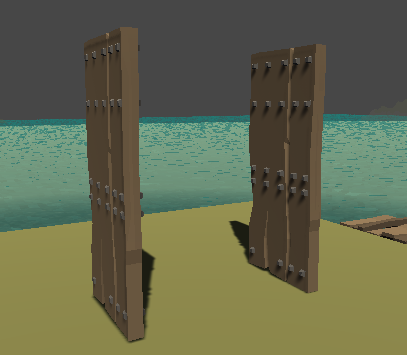
\includegraphics[scale=0.5]{doors_open.png} 
        \caption{Portes ouvertes}
    \end{subfigure}
    \hspace{50pt}
    \begin{subfigure}[t]{0.3\textwidth}
        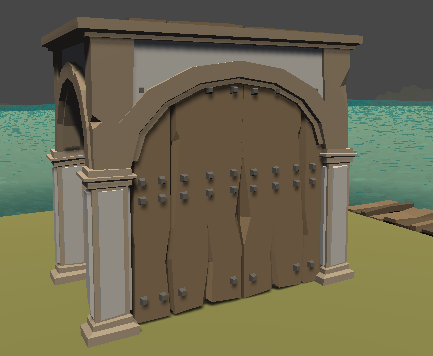
\includegraphics[scale=0.5]{doors_closed.png}
        \caption{Porte fermée avec arche}
    \end{subfigure}
    \caption{Exemple des portes que nous avons réalisé}
\end{figure}

\end{document}